\documentclass[tikz,border=8pt]{standalone}
% Shared look for every TikZ diagram. Load with % Shared look for every TikZ diagram. Load with % Shared look for every TikZ diagram. Load with \input{../../tools/tikz-style.tex}
\usepackage[T1]{fontenc}
\usepackage{lmodern}
\renewcommand{\sfdefault}{lmr}  % diagrams use the same serif as the text
\usetikzlibrary{arrows.meta, positioning, shapes.geometric, calc, fit, backgrounds}
\definecolor{cblue}{HTML}{4C78A8}
\definecolor{corange}{HTML}{F58518}
\definecolor{cgreen}{HTML}{54A24B}
\definecolor{cred}{HTML}{E45756}
\definecolor{cpurple}{HTML}{B279A2}
\definecolor{cgrey}{HTML}{6B6B6B}
\tikzset{
  every picture/.style={font=\sffamily, line width=1.2pt},
  box/.style={draw=#1, fill=#1!12, rounded corners=4pt, align=center, inner sep=7pt, minimum height=1.1cm},
  box/.default=cgrey,
  arrow/.style={-{Stealth[length=3mm]}, draw=cgrey, line width=1.4pt},
  title/.style={font=\sffamily\bfseries\Large},
  note/.style={font=\sffamily\small, text=cgrey, align=center},
}
\AtBeginDocument{\hyphenpenalty=10000 \exhyphenpenalty=10000}

\usepackage[T1]{fontenc}
\usepackage{lmodern}
\renewcommand{\sfdefault}{lmr}  % diagrams use the same serif as the text
\usetikzlibrary{arrows.meta, positioning, shapes.geometric, calc, fit, backgrounds}
\definecolor{cblue}{HTML}{4C78A8}
\definecolor{corange}{HTML}{F58518}
\definecolor{cgreen}{HTML}{54A24B}
\definecolor{cred}{HTML}{E45756}
\definecolor{cpurple}{HTML}{B279A2}
\definecolor{cgrey}{HTML}{6B6B6B}
\tikzset{
  every picture/.style={font=\sffamily, line width=1.2pt},
  box/.style={draw=#1, fill=#1!12, rounded corners=4pt, align=center, inner sep=7pt, minimum height=1.1cm},
  box/.default=cgrey,
  arrow/.style={-{Stealth[length=3mm]}, draw=cgrey, line width=1.4pt},
  title/.style={font=\sffamily\bfseries\Large},
  note/.style={font=\sffamily\small, text=cgrey, align=center},
}
\AtBeginDocument{\hyphenpenalty=10000 \exhyphenpenalty=10000}

\usepackage[T1]{fontenc}
\usepackage{lmodern}
\renewcommand{\sfdefault}{lmr}  % diagrams use the same serif as the text
\usetikzlibrary{arrows.meta, positioning, shapes.geometric, calc, fit, backgrounds}
\definecolor{cblue}{HTML}{4C78A8}
\definecolor{corange}{HTML}{F58518}
\definecolor{cgreen}{HTML}{54A24B}
\definecolor{cred}{HTML}{E45756}
\definecolor{cpurple}{HTML}{B279A2}
\definecolor{cgrey}{HTML}{6B6B6B}
\tikzset{
  every picture/.style={font=\sffamily, line width=1.2pt},
  box/.style={draw=#1, fill=#1!12, rounded corners=4pt, align=center, inner sep=7pt, minimum height=1.1cm},
  box/.default=cgrey,
  arrow/.style={-{Stealth[length=3mm]}, draw=cgrey, line width=1.4pt},
  title/.style={font=\sffamily\bfseries\Large},
  note/.style={font=\sffamily\small, text=cgrey, align=center},
}
\AtBeginDocument{\hyphenpenalty=10000 \exhyphenpenalty=10000}

\begin{document}
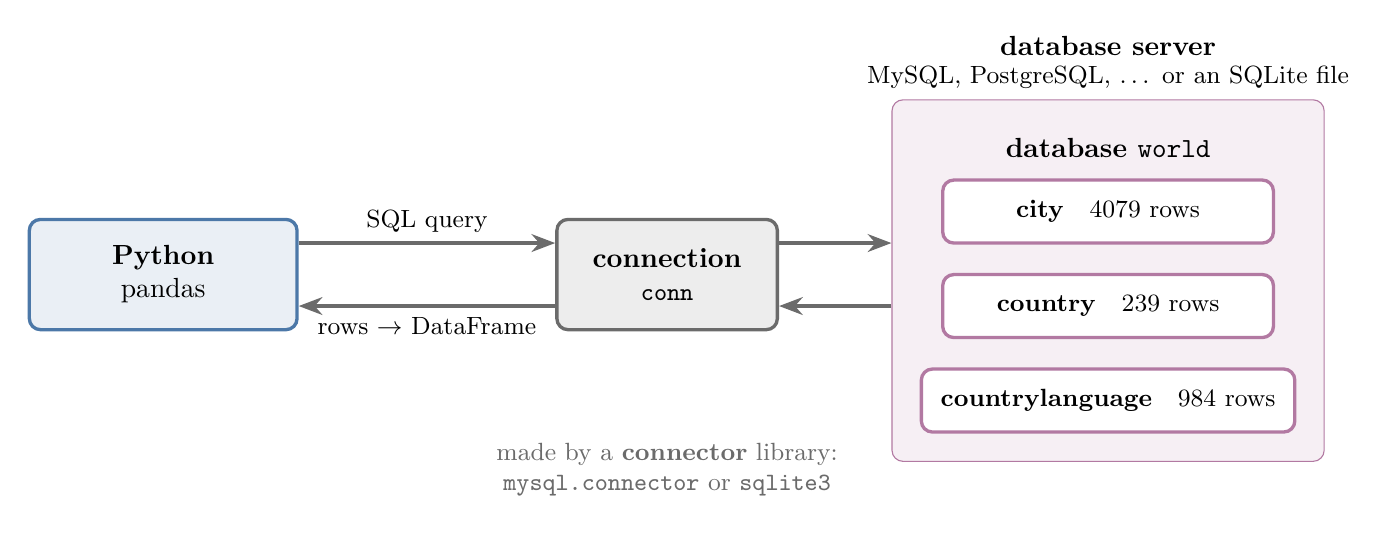
\begin{tikzpicture}
  \tikzset{tbl/.style={box=cpurple, fill=white, minimum width=4.2cm, minimum height=0.8cm, font=\small}}
  % the database server, holding the database 'world' and its three tables
  \node[tbl] (t1) at (12,0.2)  {\textbf{city}\quad 4079 rows};
  \node[tbl] (t2) at (12,-1.0) {\textbf{country}\quad 239 rows};
  \node[tbl] (t3) at (12,-2.2) {\textbf{countrylanguage}\quad 984 rows};
  \node[anchor=south, font=\sffamily\bfseries] (wl) at (12,0.75) {database \texttt{world}};
  \begin{scope}[on background layer]
    \node[box=cpurple, fit=(t1)(t3)(wl), inner sep=10pt] (db) {};
  \end{scope}
  \node[anchor=south, font=\sffamily\bfseries, align=center] at (db.north) {database server\\[-2pt]\normalfont\small MySQL, PostgreSQL, \dots\ or an SQLite file};
  % Python side
  \node[box=cblue, minimum width=3.4cm, minimum height=1.4cm] (py) at (0,-0.6) {\textbf{Python}\\pandas};
  \node[box=cgrey, minimum width=2.8cm, minimum height=1.4cm] (con) at (6.4,-0.6) {\textbf{connection}\\\small\texttt{conn}};
  \draw[arrow] ([yshift=4mm]py.east) -- node[above, font=\small]{SQL query} ([yshift=4mm]con.west);
  \draw[arrow] ([yshift=4mm]con.east) -- ([yshift=4mm]con.east -| db.west);
  \draw[arrow] ([yshift=-4mm]con.east -| db.west) -- ([yshift=-4mm]con.east);
  \draw[arrow] ([yshift=-4mm]con.west) -- node[below, font=\small]{rows $\rightarrow$ DataFrame} ([yshift=-4mm]py.east);
  \node[note, anchor=north, text width=4.4cm] at (con.south |- 0,-2.6) {made by a \textbf{connector} library:\\\texttt{mysql.connector} or \texttt{sqlite3}};
\end{tikzpicture}
\end{document}
